
\centering
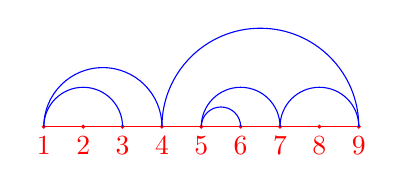
\begin{tikzpicture}[scale=0.5]


\foreach \i in {1,...,8} {
        \draw[red] (\i,1) -- (\i + 1,1)node[pos=0.0,below] {\i};
        \filldraw[red] (\i,1) circle (1pt);


 }

\draw[red] (9,1) -- (8,1)node[pos=0.0,below] {9};
\filldraw[red] (9,1) circle (1pt); 



\draw[blue, thin] (1,1) arc(180:0:1); 
\draw[blue, thin] (1,1) arc(180:0:1.5);
\draw[blue, thin] (4,1) arc(180:0:2.5); 
\draw[blue, thin] (5,1) arc(180:0:0.5); 
\draw[blue, thin] (5,1) arc(180:0:1);
\draw[blue, thin] (7,1) arc(180:0:1);

\end{tikzpicture} 